\chapter{User interface design}
\label{chap:user_interface_design}
\section{Method}

\subsection{Iterative design}
When designing a user interface with the intention of reaching a high level of usability, a systematic approach is key. The process we have used, can be roughly divided in to 4 steps, where the latter part can be repeated until the Quality Requirements, listed in \ref{subsec:quality_requirements}, have been met. \cite{lauesen} \\
The steps are:
\begin{enumerate}
\item Analysis of users and tasks
\item Construct prototype
\item Perform usability tests
\item Amend prototype 
\end{enumerate}

The semester planning and day to day booking have been described seperately, due to the differences between them. We will provide a detailed walkthrough of the process for an element in each part, and the full history of mockups can be found in appendix \ref{app:mockups}.

\subsection{Usability testing}
\label{sec:usability_testing}
Choosing which, and how many, test subjects is needed for a test is a heavily debated subject in the usability community. Most tend to agree that 5 or below is more than enough for each round. The controversy arise when figuring out how representative the test subjects most be for your target audience. Soren Lauesen opens the corresponding chapter with: \cite{lauesen}
\begin{quotation}
\noindent \emph{``A usability test must of course be made with users that correspond to the real users we expect in practice.''}
\end{quotation}
However, Steve Krug has a different view: \cite{steve}
\begin{quotation}
\noindent \emph{``The importance of recruiting representative users is overrated. [...]''} \\
\noindent \emph{``The best-kept secret of usability testing is the extent to which it doesn't much matter who you test.''}
\end{quotation}

What we can take away from their different arguments for and against, is that testing with representative users is \emph{good}, but not vital when it simply comes to eliminating problems.
We have chosen to do both. The system is intended to be used by everyone at ITU, which will also include newly started students and faculty.
Another point of agreement among the experts, is that testing early and often will \emph{always} trumps testing with many users at a later point. \cite{lauesen,steve,nielsen_five_users}

The table in figure \ref{fig:usa_users} shows how many users have been tested for each part of the system for each round. As seen, we've opted to only test one user for the semester planning, which is simply due to the lack of people with the required knowledge, and the very narrow target audience.

\begin{figure}[htb]
\begin{center}
\leavevmode
	\begin{tabular}{|l|r|r|r||r|}
		\hline
		 & Round 1 & Round 2 & Round 3 & Total \\ \hline
		Day to day & 2 & 2 & 2 & 6\\ \hline
		Semester & 1 & 1 & n/a & 2 \\ \hline
	\end{tabular}
\end{center}
\caption{Overview of test users per round}
\label{fig:usa_users}
\end{figure}

The results from our tests can be found in the following sections, whereas the full test documentation can be found in appendix \ref{app:tests}.

\section{Day to day booking}
\label{sec:day_to_day_booking_ui}
As described in previous chapters, the day to day booking should be usable without any instructions. We have tried to imitate familiar designs, and use common design conventions. As Steve Krug puts it\cite{steve}: 
\begin{quotation}
\emph{``All conventions start life as somebody's bright idea. If the idea works will enough, other sites imitate it and eventually enough people have seen it in enough places that it needs no explanation.''}
\end{quotation}

\subsection{Wireframe}
\label{subsec:wireframe}
\todo{relevance? rename/move/divide}
The front page serves as a portal to the rest of the system, and thus it should be easy to understand. To ensure that we had the vital navigation functions in place before beginning the mockups, we constructed a wireframe\cite{garrett}. The wireframe, as seen on figure \ref{fig:wireframe_frontpage}, has the following elements:

\begin{figure}[htb]
\begin{center}
\leavevmode
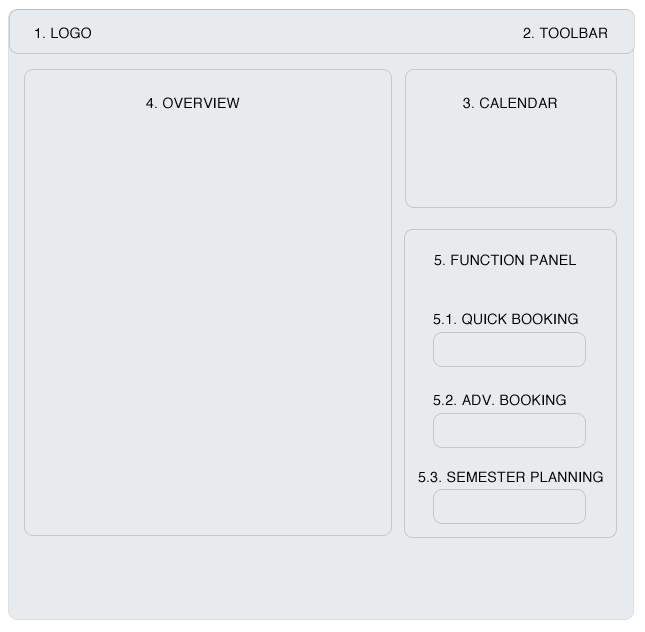
\includegraphics[width=0.6\textwidth]{images/wireframe1}
\end{center}
\caption{Wireframe for the frontpage}
\label{fig:wireframe_frontpage}
\end{figure}

\begin{itemize}
	\item \textbf{1. Logo}\\
	The logo for the application, which by convention should be located in the top left corner and link to the frontpage. \cite{steve}
	\item \textbf{2. Toolbar}\\
	A navigation toolbar. Should be used to login and logout, and for accessing the personal user account overview.
	\item \textbf{3. Calendar}\\
	An object used to navigate to a specific day in the future (or past).
	\item \textbf{4. Overview}\\
	The main overview, which should present a map of the university.
	\item \textbf{5. Function panel}\\
	A panel containing buttons used to enter the booking interface, or the semester planning.
\end{itemize}


\subsection{Test results}

\subsection{Design process}
\label{sec:design_process}

\subsubsection{Design of the day to day booking interface}
For a full history of our mockups, please refer to %\ref{app:mockups}

\begin{figure}[htb]
\begin{center}
\leavevmode
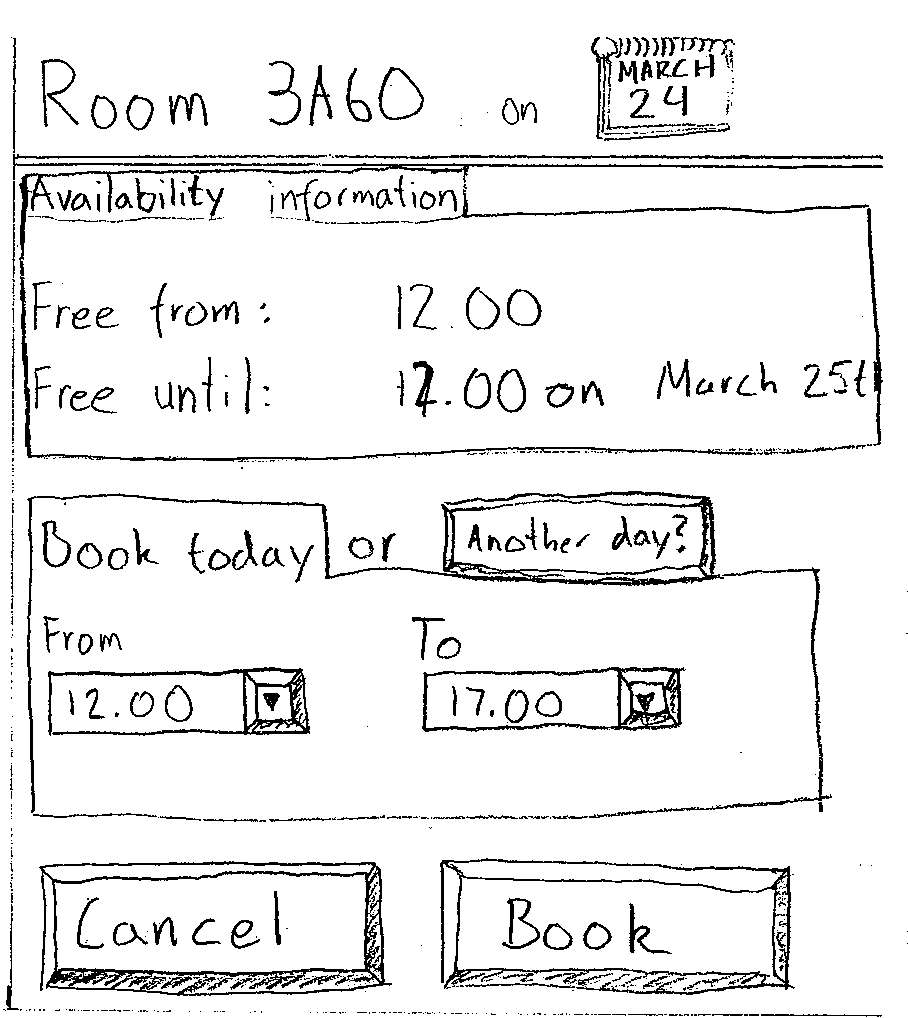
\includegraphics[width=0.6\textwidth]{images/bookRoomMockup}
\end{center}
\caption{First draft of the simple booking panel}
\label{fig:book_room_mockup}
\end{figure}

Seen on figure \ref{fig:book_room_mockup} is the function of the main screen, which was thought to be in charge of all interaction, trying to give the user the impression that they never left the homepage, and to make sure no-one got lost in subscreens and menus. Our first usability tests quickly revealed that we had been mistaken. All the test subjects felt overwhelmed by the amount of options, and due to all the clutter did not spot the vital functions.

\begin{figure}[htb]
\begin{center}
\leavevmode
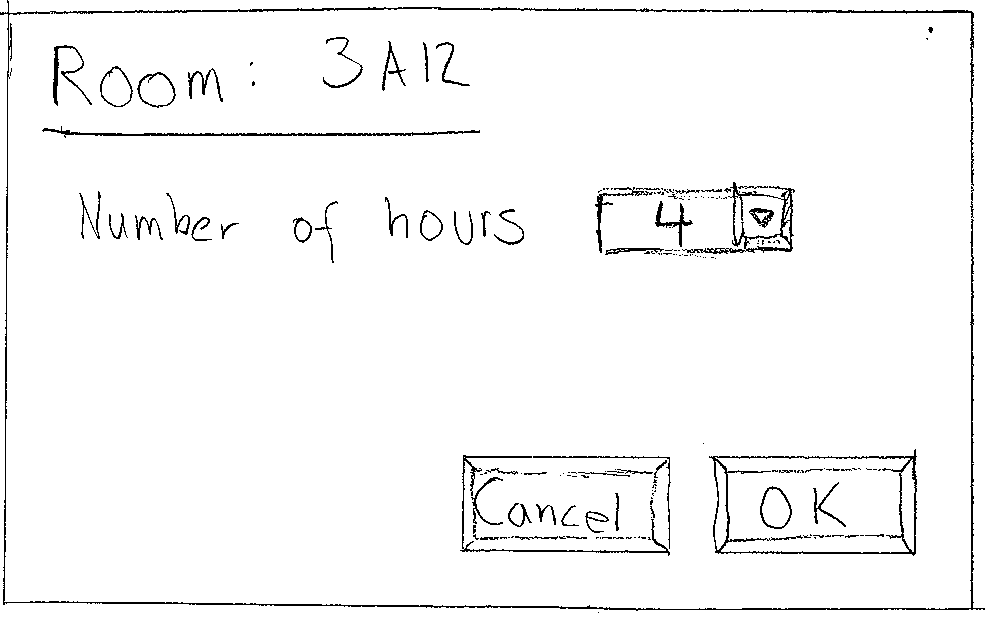
\includegraphics[width=0.8\textwidth]{images/bookRoomMockup2}
\end{center}
\caption{Second attempt at the simple booking. This time as a window overlaying the main view.}
\label{fig:book_room_mockup2}
\end{figure}

Second time around, we tried making it as basic as possible and simply presenting the user with a dialog (not a pop-up, just an overlay) for selecting how many hours from now the room should be booked. The flaw with this was that noone was able to figure out the availability of a room in the near future. This is when we realized that the best successes we've had with room booking was the first draft of the week-overview screen.

\begin{figure}[htb]
\begin{center}
\leavevmode
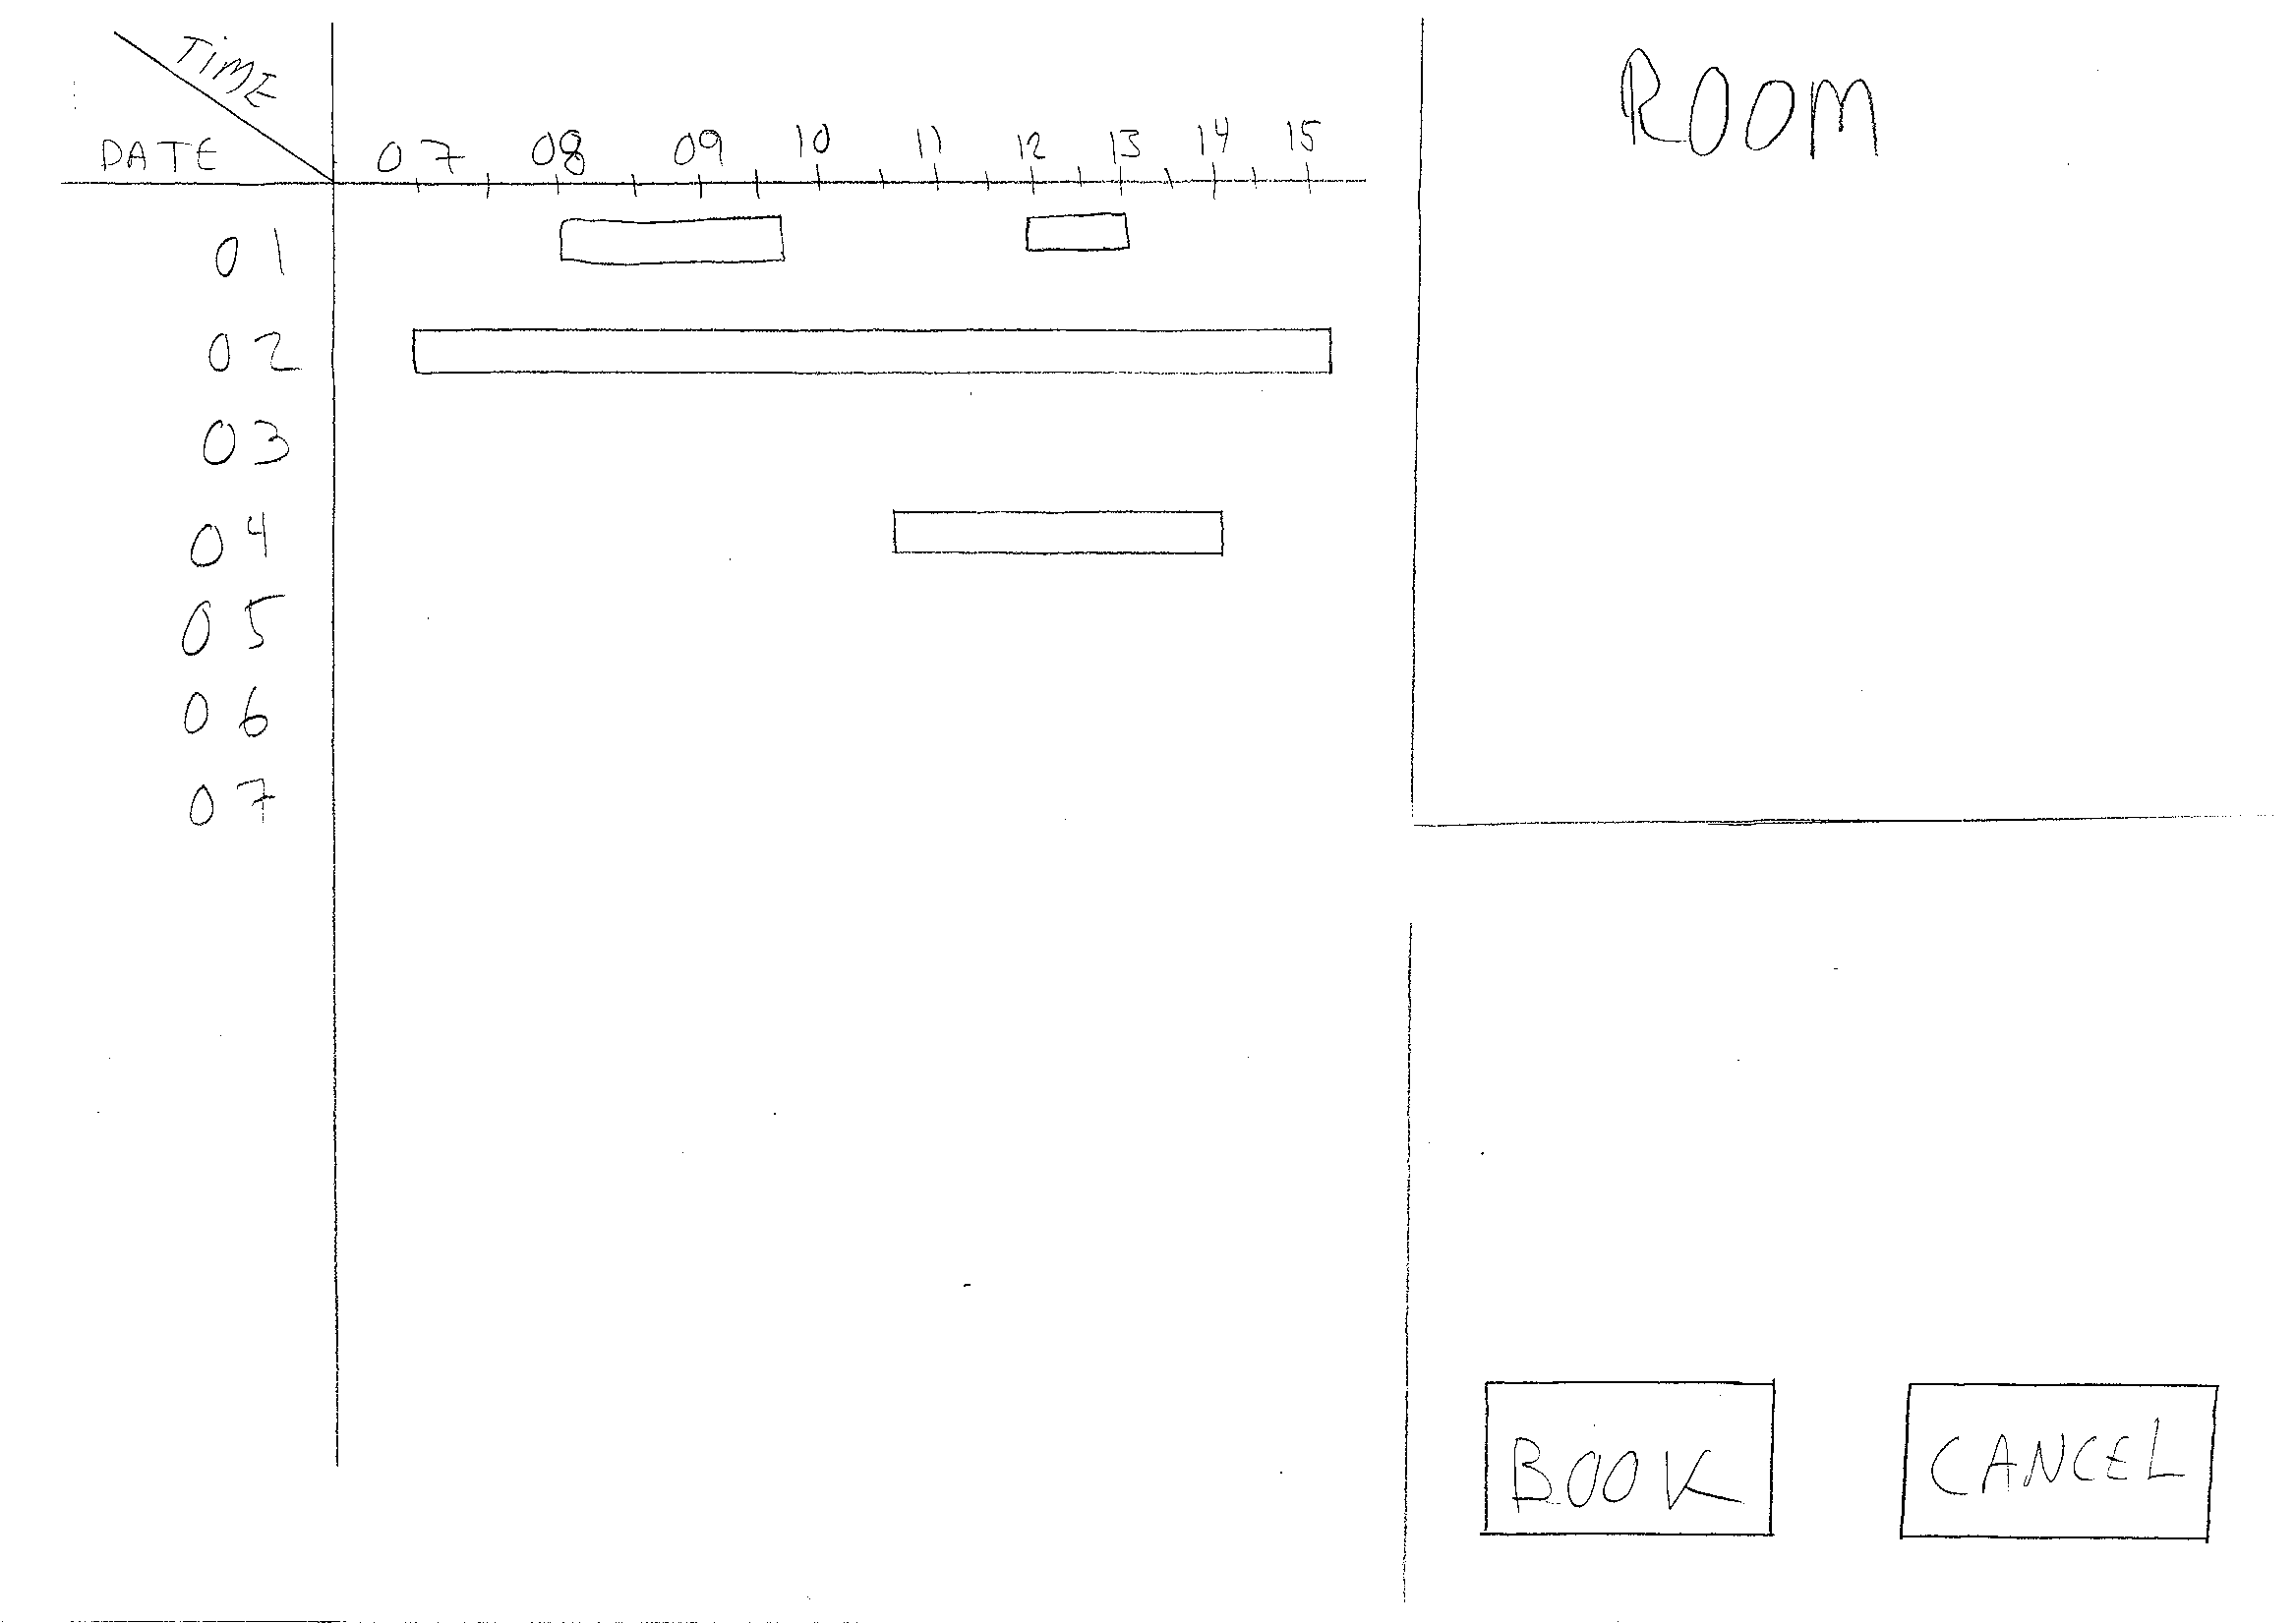
\includegraphics[width=0.8\textwidth]{images/weekMockup}
\end{center}
\caption{The mockup screen for a week overview on a specific room.}
\label{fig:week_mockup}
\end{figure}

All the test subjects used the 'matrix' overview shown on figure \ref{fig:week_mockup} both creatively and effectively, so we decided to try and utilize that success to the maximum by redirecting even a simple booking task to the same screen.
The only exception we have made to this is when using the "book now"-functionality, which will simply book a room for 4 hours and notify the user which one they have been assigned, with the ability to either accept or reject.

\begin{figure}[htb]
\begin{center}
\leavevmode
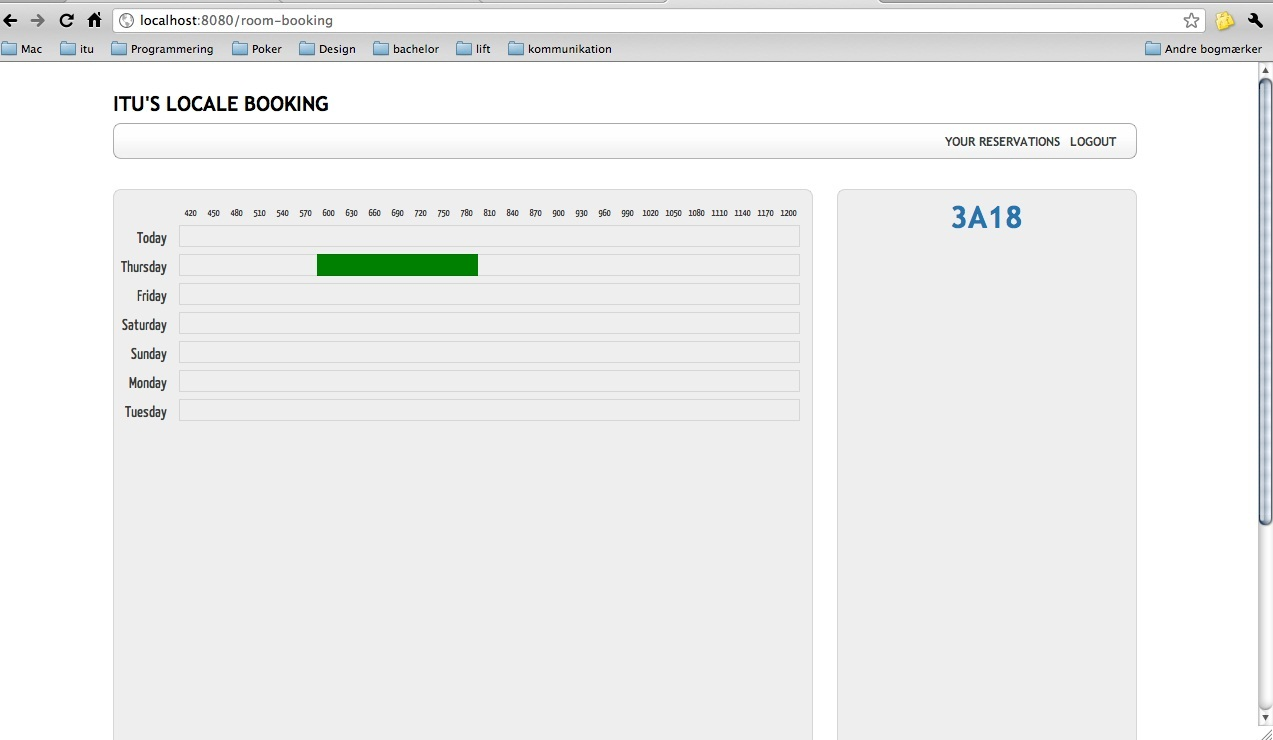
\includegraphics[width=1\textwidth]{images/weekFinal}
\end{center}
\caption{The almost finished screen for a week overview on a specific room.}
\label{fig:week_final}
\end{figure}

The final design to book a room, as shown on figure \ref{fig:week_final}, grants an availability overview of 7 days, starting with the current day. Through our tests, we noted test subjects trying to drag the mouse to select, and others clicking for a start time followed by a click on end time, so we have chosen to allow for both.
To assist the user in figuring out how it works, we have added highlighting of both the day and time when mouse is moved across the matrix.

Søren Lauesens first law of usability\cite{lauesen} states that a heuristic evaluation of usability flaws only has a 50\% hit-rate, which we admittedly found out was the case. We anticipated that our first design might be too dense, but never guessed that the wider overview proved more efficient for a simple booking.
\todo{fix it}


\subsection{Proposed design}
\label{sec:proposed_design}
\todo{Explain and illustrate the proposed design}

\section{Semester planning}
\label{sec:semester_planning_ui}
